\documentclass[10pt,twocolumn,letterpaper]{article}

\usepackage{cvpr}
\usepackage{times}
\usepackage{epsfig}
\usepackage{graphicx}
\usepackage{amsmath}
\usepackage{amssymb}
\usepackage{wrapfig}

% Include other packages here, before hyperref.

% If you comment hyperref and then uncomment it, you should delete
% egpaper.aux before re-running latex.  (Or just hit 'q' on the first latex
% run, let it finish, and you should be clear).
\usepackage[pagebackref=true,breaklinks=true,letterpaper=true,colorlinks,bookmarks=false]{hyperref}

\cvprfinalcopy % *** Uncomment this line for the final submission

\def\cvprPaperID{1} %
\def\httilde{\mbox{\tt\raisebox{-.5ex}{\symbol{126}}}}

% Pages are numbered in submission mode, and unnumbered in camera-ready
\ifcvprfinal\pagestyle{empty}\fi

\begin{document}

%%%%%%%%% TITLE
\title{Practical AutoAugment: Measuring the Impact of AutoAugment on Classification Performance Across Image Datasets}

\author{Quoc N. Le, Rounak Mehta, Vikram Natarajan, Anna Novakovska\\
Columbia University\\
{\tt\small \{qnl2000,rm3652,vsn2113,an2915\}@columbia.edu}
\\
}

\maketitle
%\thispagestyle{empty}

%%%%%%%%% ABSTRACT
\begin{abstract}
The AutoAugment [1] authors show how automatically-selected policies for data augmentation can improve on benchmark classifier performance on CIFAR-10, CIFAR-100, SVHN, and other datasets.  In this paper, we put ourselves in the shoes of practitioners seeking to use AutoAugment to improve image classification performance on their own real-world datasets.

The first practical approach to unlocking the value of AutoAugment is to "transfer" augmentation policies found on one dataset onto other datasets. This worked well for the datasets in the AutoAugment paper, but we report mixed results for using transfer learning approach on two additional image datasets: the “Iceberg” dataset from the Kaggle “Statoil/C-CORE Iceberg Classifier Challenge" and the "QuickDraw" dataset from the Kaggle "Quick, Draw! Doodle Recognition Challenge".  For the Iceberg dataset we achieved immediate gains by (1) transfering CIFAR-10 policies which resulted in a 2.6 percent improvement in log loss of our baseline, (2) transfering SVHN policies directly which resulted in a 5.1 percent improvement over our baseline, and (3) transfering manually selected SVHN policies which resulted in a 15.1 percent improvement over our baseline.  For the QuickDraw dataset, however, we did not measure any gains, in fact we struggled to improve our baseline using augmentation (although there may be problems with our experiment which caused this).  Our conclusion is that gains from transfer learning using AutoAugment depends on the dataset, although the gains can be impressive and very straightforward as they were with the Iceberg dataset.  Therefore, practitioners should certainly consider AutoAugment transfer in their model optimization.

The second approach to unlocking value in AutoAugment is to leverage the AutoAugment [1] reinforcement learning framework to discover optimal policies on any target dataset.  We found, however, that it is difficult to reproduce the reinforcement learning implementation described in the paper, due to lack of detail in the AutoAugment paper.  We instead developed an approach we call Simplified AutoAugment, where we implemented a “Random Search Controller” which is a simplification on the Reinforcement Learning Controller [1] and also suggested by the AutoAugment authors.  We find that our Random Search Controller is able to achieve 3.33 percent error on the CIFAR-10 Wide-Res-Net benchmark, which is an improvement on the no-augmentation baseline of 3.87 percent.  However, the Random Search Controller does not produce policies as optimal as the Reinforcement Learning Controller, which has a 2.68 percent error rate.  Still, we conclude that an Random Search approach can provide a practical alternative for practitioners to automatically find augmentation policies that improve on a classifier baseline.

\end{abstract}

%%%%%%%%% BODY TEXT
\section{Introduction}

AutoAugment shows the potential for automatically discovering data augmentation techniques that can be “learned” from the image dataset itself. It is a reinforcement learning algorithm which finds optimal policies for data augmentation for training deep learning algorithms. It works by setting the problem up as a discrete search problem, where each policy in the search space corresponds to five sub-policies (each having 2 operations). Reinforcement Learning is used to find optimal policies, then these policies are used to augment a dataset before training with a selected neural network architecture.

The original AutoAugment paper [1] demonstrated the performance of AutoAugment on benchmark datasets such as CIFAR-10, CIFAR-100, SVHN, and ImageNet, and also showed that learned policies do transfer to other target datasets.  That is, the optimal augmentation policies learned to optimize classifier performance on one image dataset will “transfer” or improve classifier performance on a different dataset.   We will measure this transferability onto additional datasets, in particular the Iceberg and QuickDraw datasets described in a subsequent section.  These results are summarized in the "Results - Transfer Learning” section.

However, to learn these policies, the authors use a Reinforcement Learning algorithm whose implementation is not made available with their paper [1].  Therefore we experiment with a "Simplified AutoAugment" approach, where we search over the space of possible policies using a Random Search.  This is a simplified approach because we avoid the complexities of implementing the Reinforcement Learning, although the trade off is likely a smaller positive impact on classifier performance.  Nonetheless, the Random Search is suggested by the AutoAugment [1] authors as a possible research direction that could yield competitive results to Reinforcement Learning. These results are summarized in the "Results - Simplified AutoAugment” section.

\section{Previous Work}

The original AutoAugment paper [1] has a github project that shows the application of the discovered augmentation policies to training the classifiers for CIFAR-10 and CIFAR-100.  There are also a number of github repositories that attempt to reproduce the results of the original paper (DeepVoltaire/AutoAugment, rpmcruz/autoaugment, dnddnjs/pytorch-cifar10).  However, none of these repositories successfully provides an implementation that reproduces the results of the Reinforcement Learning algorithm of the original paper.

The rpmcruz/AutoAugment github repository [3], however, provides the most useful attempted implementation of the Reinforcement Learning approach in the original paper.  This repo leverages the Reinforcement Learning implementations details from two papers [1-2], and in doing so it at least provides a Controller and Child framework for policy searches, where the Controller suggests policies while the Child tests the effect of the policy on training the network.  This was useful to us as we could plug in experimental Controllers that perform a Random Search of policies, for example.

Findings show that random search can provide competitive approach to reinforcement learning [4], however it was not compared with AutoAugment.

\section{Datasets}

We chose image datasets from Kaggle based on the following criteria:

\begin{itemize}
  \item Image dataset is labeled, i.e. classification is the goal
  \item Image dataset is of a manageable size (less than 20GB)
  \item Existence of a Kaggle Kernel which provides a classifier baseline for the dataset.  A Kaggle Kernel is a replayable script that runs in a controlled environment on the Kaggle platform.  This ensures easy reproducibility of the baseline, since both the code and runtime environment for the model training and evaluation is provided.
  \item Kernel is a single model that can be run relatively quickly (under 12 hours).  Note this excludes many competition-winning models which are large ensembles and take days to run.
\end{itemize}

The datasets that met these criteria include:

\begin{itemize}
  \item \textbf{Iceberg Dataset}.  This is an image dataset from the Kaggle “Statoil/C-CORE Iceberg Classifier Challenge".  It contains 1,674 "images" of icebergs and ships that come from radar readings.  
  \item \textbf{QuickDraw Dataset}.  This is an image dataset from the Kaggle “Quick, Draw! Doodle Recognition Challenge".  It contains over 50 million images of doodles (quick drawings) which belong to 340 categories.  
  \item \textbf{CIFAR-10 Dataset}.  This is the same canonical dataset used by the authors [1].  We use this for comparing the Simplified AutoAugment performance to that of the Reinforcement Learning AutoAugment.  Although this dataset is not a Kaggle dataset, it is labeled, relatively small, and has many classifier baselines as specified in the AutoAugment paper [1].        
\end{itemize}


\section{Evaluation Criteria}

\subsection{Transfer Learning}

To measure \textbf{Transfer Learning} on augmentation policies, we will evaluate the following on the Iceberg and QuickDraw datasets:

\begin{itemize}
  \item Performance of the classifier baseline (Kaggle Kernel) without any data augmentation.  This will require removing and data augmentation added by the Kernel author, if any.  We will describe the baselines in more detail in the Results sections.
  \item Performance of the classifier with data augmentation policies discovered by AutoAugment for CIFAR-10 and SVHN.  We are hoping for a clear improvement over the baseline above.
  \item Performance of the classifier with data augmentation policies using a subset of the AutoAugment policies SVHN.  We would like to know whether performance improvements over using full augmentation policies is possible.
\end{itemize}

The definition of "Performance" will depend on the dataset.  For Iceberg, the performance measure will be Binary Log Loss.  The performance metric for the QuickDraw competition (and our chosen MobileNet baseline) is Mean Average Precision @3 (MAP@3), a custom metric defined for the competition described here https://bit.ly/2Q0jqH7.

\subsection{Simplified AutoAugment}

To measure the effectiveness of our \textbf{Simplified AutoAugment} policies, we will compare to accuracy of Wide-ResNet-28-10 using AutoAugment [1] policies on CIFAR-10.  Specifically we will compare:

\begin{itemize}
  \item Reported accuracy of the classifier baseline (Wide-ResNet-28-10) without any data augmentation, as reported in the AutoAugment paper [1].  This was reported as 3.87 percent error.
  \item Our own measured performance of the CIFAR-10 Wide-ResNet-28-10 baseline with data augmentation policies discovered for the dataset by AutoAugment using Reinforcement Learning.  We will seek to reproduce the reported percent error of 2.68 from the AutoAugment paper [1].
  \item Our measured performance of the  CIFAR-10 Wide-ResNet-28-10 baseline with data augmentation policies discovered for the dataset by our Simplified AutoAugment which uses Random Search instead of Reinforcement Learning.  
\end{itemize}

We would expect the performance of Simplified AutoAugment to fall somewhere between 3.87 and 2.68 percent, but our experiment will reveal where in the spectrum it falls.


\section{Results - Transfer Learning}

\subsection{Iceberg Dataset}

After adding AutoAugment transfer augmentations to “Statoil/C-CORE Iceberg Classifier” Kaggle Dataset, we got 2942 examples (an increase over the original 1,674 images). All the images are 75x75 images with 2 Channels and 2 classes (iceberg/ship).  These "images" are actually radar readings so are not in fact pictures,  but they can be visualized in 3D as follows:

\begin{figure}[bhp]
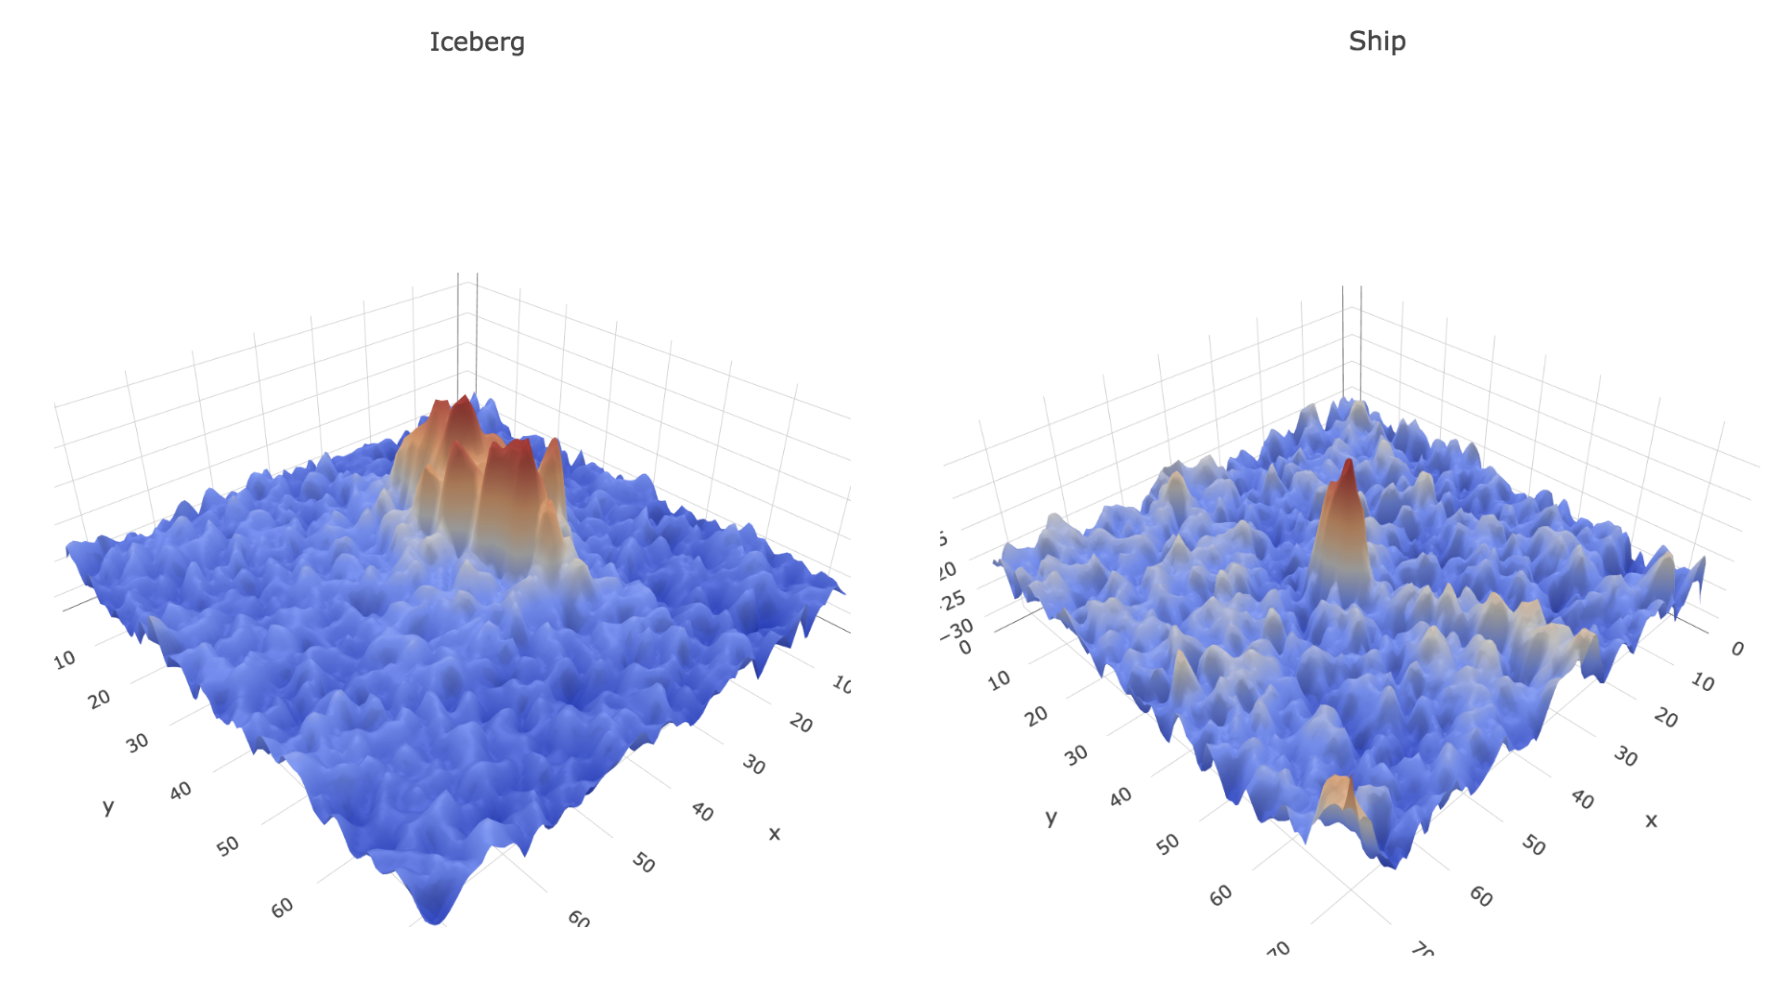
\includegraphics[width=\columnwidth]{iceberg_ship_example.png}
\caption{Iceberg and Ship examples from dataset.}
\end{figure}

We can also visualize the augmented images in 3D as well.  The following example shows an augmented image based on a ShearY+Rotate transformation.  This means that the image was sheared along the vertical axis, and in addition it was rotated.  The shear is a little hard to see but the rotation is clear.

\begin{figure}[bhp]
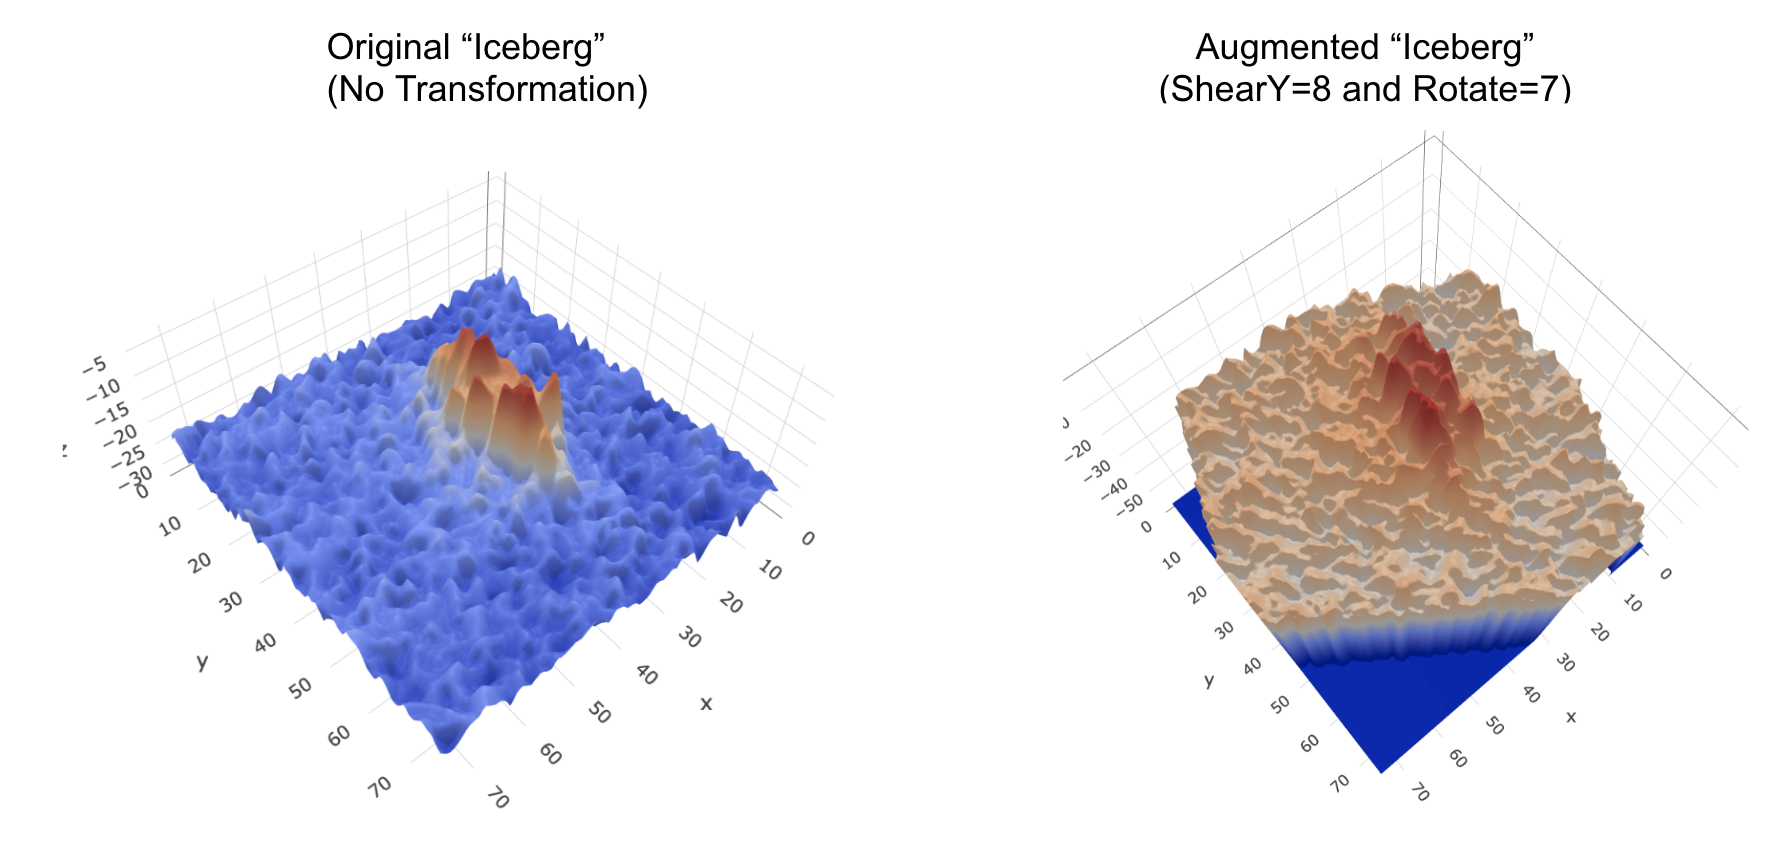
\includegraphics[width=\columnwidth]{iceberg_aug_example.png}
\caption{Visualizing Iceberg Augmentation in 3D.  The original image is on the left and the augmented Shear+Rotate image is on the right.}
\end{figure}

The neural network only operates on 2D images, however.  Below is an example of the representation that the neural network would actually work with.

\begin{figure}[bhp]
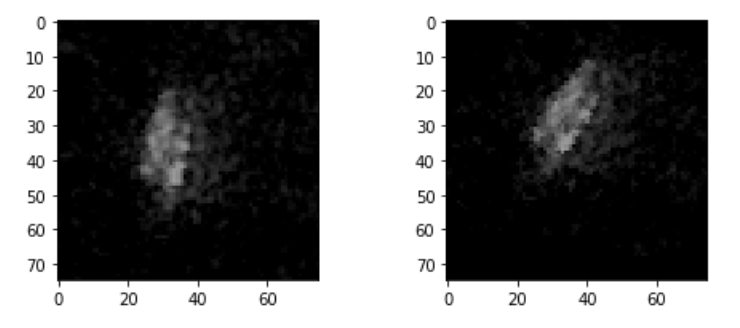
\includegraphics[width=\columnwidth]{iceberg_aug_2d_example.png}
\caption{Visualizing Iceberg Augmentation in 2D.  The original image is on the left and the augmented Shear+Rotate image is on the right.}
\end{figure}

Moving onto network architecture, the model came from a Kaggle Kernel called "My Best Single Model - Simple CNN" by Jirka Vrany [6].  It uses a CNN model that was one of the best single models in the above Iceberg competition. The architecture is comprised of 2 consecutive Convolution blocks with 3 Convolutional layers and 1 Max Pooling layer, followed by 2 Convolution blocks with 1 Convolution layer and 1 Max Pooling layer. It is followed by 3 Dense layers with dropouts. It uses Adam optimizer with no weight decay and learning rate 0.0001. Model was trained for 30 epochs on each fold, producing 10 models which were ensembled into a final model.  

We again note that there were certainly better-performing baseline classifiers in the Kaggle Iceberg competition, but for this paper we preferred simple, single models that can run in a reasonable amount of time.

The baseline model described above (trained with no augmentation) scored log loss of 0.1446 on the competition's public holdout set. (This was actually better than the reported 0.1541 log loss on the public competition holdout set, and this was due to our removing the author's hand-selected augmentations).  Using the exact augmentation policies from the original paper [1], we achieve an log loss of 0.1409 using CIFAR-10 augmentations and 0.1376 using SVHN augmentations.  These are significant improvements of 2.6 percent and 5.1 percent respectively.  The results are shown below.


    \begin{table}[h]
      \begin{tabular}{lll}
        \hline
        Experiment &Log Loss & Improvement   \\ \hline
        Baseline CNN (No Aug.)  &0.1446 &-\\
        w/CIFAR-10 Policies &0.1402  & 2.6\%\\
        w/SVHN Policies (Full) &0.1376  & 5.1\%\\
        w/SVHN Non-Color Policies &0.1256  &15.1\%\\  
        \hline
      \end{tabular}
      \\
      \caption{Results When Transfering CIFAR-10 and SVHN Policies to Training on Iceberg Dataset.  The Log Loss reported is on the competition public holdout set.}
    \end{table}


To understand the results above, we need to consider the nature of the Iceberg radar/image data.  The original data consists of two 75x75 matrixes with positional radar readings.  These readings are artificially transformed into 2D "images" by transforming them to a color scale between 0 and 255 and adding a 3rd channel which is just the average of the other 2.  So intuitively speaking, the height of the iceberg or ship in the radar data gets mapped to a color in the image, so the 2D image is sort of a bird's eye view of the iceberg or ship.

What then happens with any augmentation that operates on color, such as Solarize, Invert, Color, etc as shown in Table 7 of the AutoAugment paper [1].  These augmentations have the effect of changing the "height" of the iceberg or ship reading.  In the worst case, as is the case with Solarize, this results in data which will never be observed in the real world.  Consider for example what a Solarize transformation does to the original data, as shown in 3D below.


\begin{figure}[bhp]
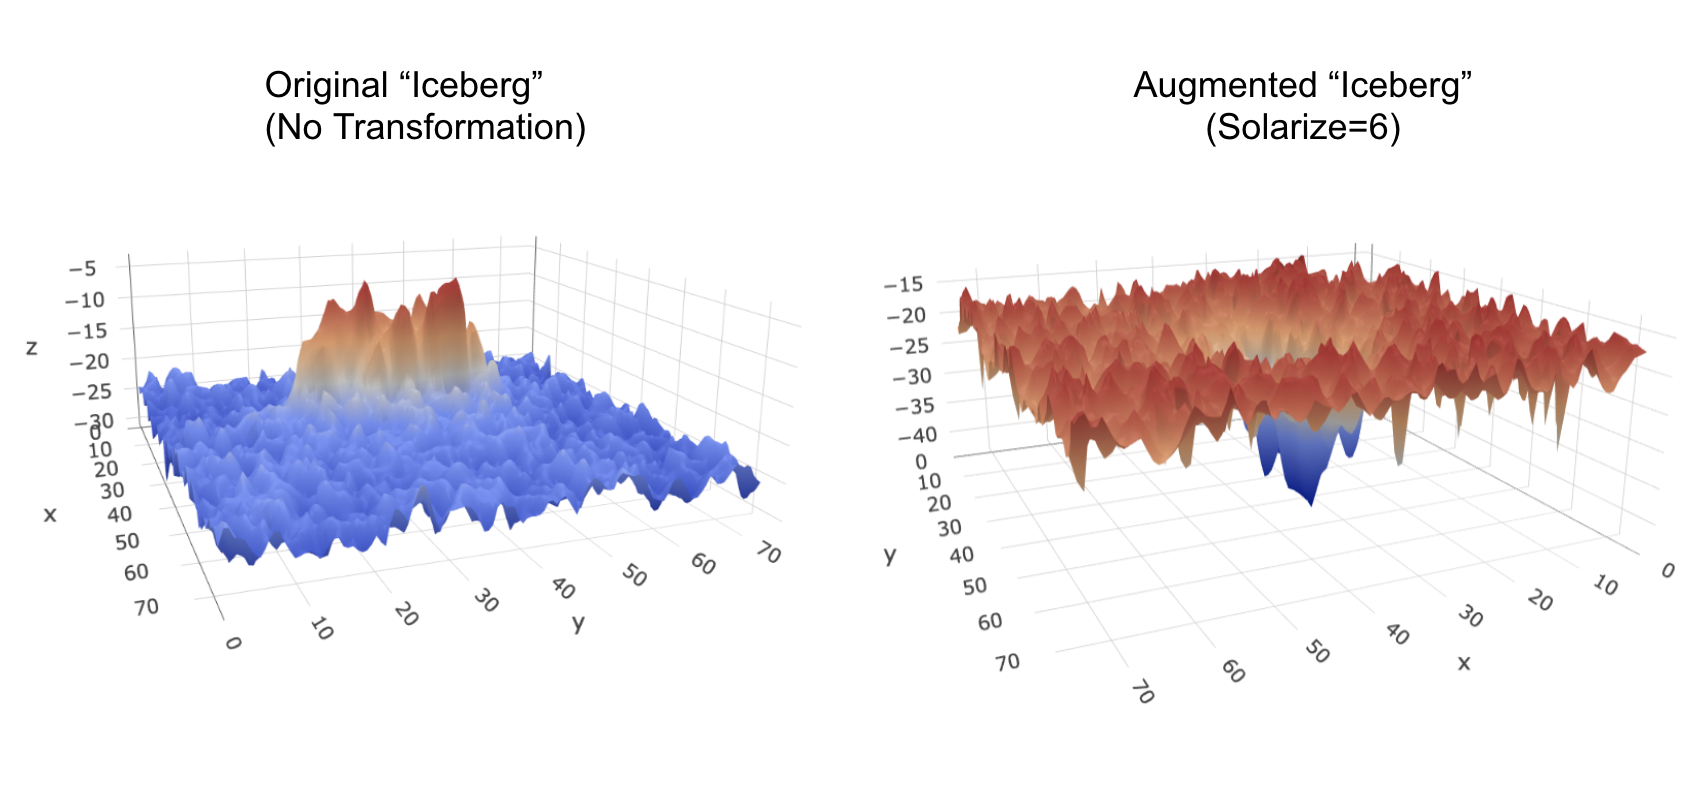
\includegraphics[width=\columnwidth]{iceberg_solarize.png}
\caption{Visualizing the Solarize transformation on an iceberg. This produces a non-helpful augmentation.}
\end{figure}

Clearly, this augmentation will not help the neural network learn, as the augmentation creates an iceberg that is upside-down relative to all the icebergs in the test data set (and in the real world).

Given this observation, the relatively small improvements from transferring CIFAR-10 policies makes sense because those policies include many color-related augmentations such as Color, Solarize, Brightness, AutoContrast, etc, as shown in Table 7 of the AutoAugment paper [1].  On the other hand, the improvements from using SVHN augmentations are almost twice as big, which makes sense because the SVHN augmentations contain relatively more positional transformations like ShearX, ShearY, Rotate, TranslateX, TranslateY, etc.

The largest improvement, however, comes when we reduce the SVHN policies by removing policies that involve Solarize, AutoContrast, and Contrast (SVHN Non-Color Policies in Table 1).  This results in a 15.1\% improvement in the baseline as shown in Table 1.  The significance of this experiment is that it shows that augmentation policies are not necessarily optimal when transferred, and that simple heuristical modifications like suppressing color-related augmentations in the transferred policies can produce a significant improvement.


\subsection{QuickDraw Dataset}

The QuickDraw is dataset is a much larger dataset than the Iceberg dataset, consisting of over 50 million images from human drawings or doodles classified into 340 classes.  Each image is 64x64 with 3 color channels.  

The baseline classifier is one based on MobileNets [7] and was created by Kaggle user Beluga [8].  The most significant aspect of the model is that it uses a preprocessor that converts the original color doodles into greyscale images before feeding those images into a MobileNet.  (This will have an impact on the effectiveness of color augmentation policies)  The Keras implementation of MobileNets is used with a learning rate of 0.002.


    \begin{table}[h]
      \begin{tabular}{lll}
        \hline
        Experiment &MAP@3    \\ \hline
        Baseline MobileNet (No Aug.) - 48 Epochs  &0.890 \\
        Baseline MobileNet (No Aug.) - 15 Epochs  &0.830 \\        
        w/CIFAR-10 Policies &0.785  \\
        w/SVHN Policies (Full) &0.806  \\
        w/SVHN Non-Color Policies &0.821  \\  
        \hline
      \end{tabular}
      \\
      \caption{Results When Transfering CIFAR-10 and SVHN Policies to Training on QuickDraw Dataset.  The Mean Average Precision (MAP@3) is measured on the competition public holdout set.}
    \end{table}



First a bit about the experiments shown in Table 2.  The Kaggle Kernel based on MobileNets is capable of scoring 0.890 on the competition public leaderboard, and we confirmed this through our own replay of the kernel which took about 8 hours.  Due to the cost of calculating data augmentations during training, however, we found that we needed to reduce the number of epochs used the MobileNet to just 15 epochs so that the experiments with augmentations could run in about 8 hours.  This baseline with 15 epochs scored 0.830, so we decided to use it as our actual baseline.

We spent considerable time trying to understand the results of these experiments shown in Table 2.  On one hand, given the images are transformed to greyscale, the scores for the augmentation experiments relative to each other make sense.  Specifically, we would expect the CIFAR-10 policies to do the worst because it contains many augmentations that are color related.  SVHN should be better because it contains more positional transformations.  Finally, the subset SVHN policies that exclude Contrast, AutoContrast, and Solarize ("Non-Color Policies") should do the relative best.

One the other hand, the scores relative to the 15 epoch baseline did not make sense initially, since we did not expect the augmentations to actually hurt baseline performance.  We offer two hypotheses next.  

First, it is possible that when we reduced the number of epochs used in the baseline to 15, this put the experiments which used augmentations at a disadvantage. There is a probabilistic nature to the application of policies in AutoAugment, so perhaps with more epochs the experiments with augmentations could overtake the baseline (assuming they run with the same number of epochs).

Next, it is likely that gains from transfer learning from data augmentations are simply not guaranteed for any dataset.  That is, the effectiveness of augmentation transfer learning is probably very dataset/algorithm/performance-metric specific.  We certainly saw in the Iceberg analysis how the Solarize transformation destroys signal as in Figure 4.  The CIFAR-10 and SVHN policies may be similarly non-optimal for the greyscale, whitespace-dominant nature of the QuickDraw images.


%\vfill\null

\section{Results - Simplified AutoAugment}

\begin{figure}[bhp]
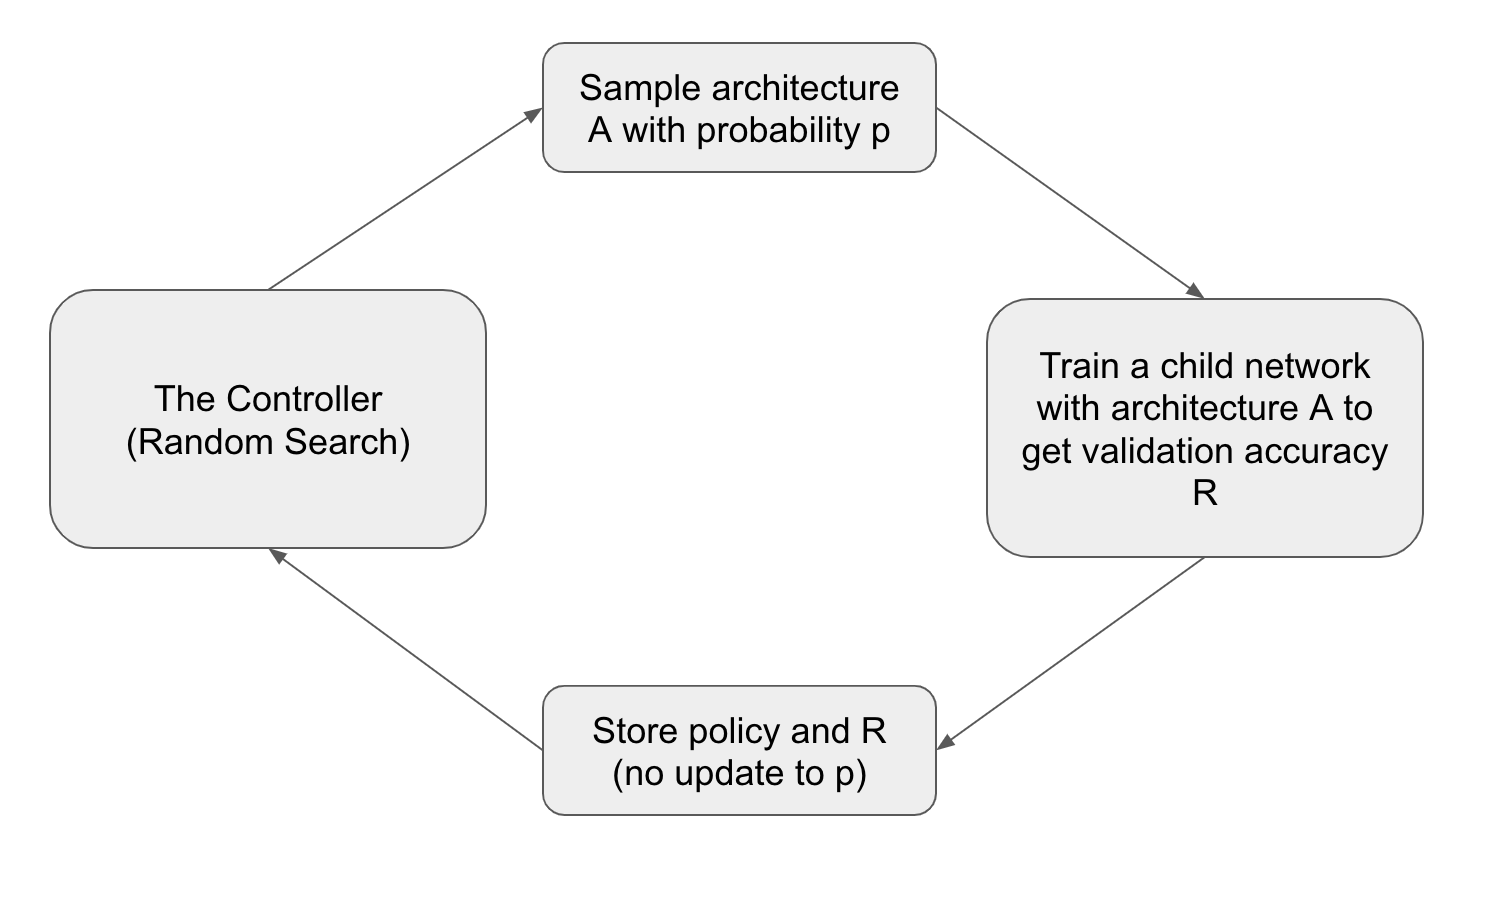
\includegraphics[width=\columnwidth]{random_search_arch.png}
\caption{Overview of policy search using a random search controller architecture.}
\end{figure}

In our original proposal, we had planned to apply the AutoAugment [1] using the same Reinforcement Learning approach for finding the best policies that was suggested in the paper.  That proved to be difficult due to insufficient details in the paper, such as the number of epochs used in the Controller.  It would also require extensive computational resources to reproduce the exact results in the paper.

An alternative strategy, shown in Figure 5, is to find good policies using a random search over the set of all possible policies. We call this the "Simplified AutoAugment".  This strategy was inspired by random grid search for hyperparameter tuning, and it is much simpler than Reinforcement Learning LSTM Controller described in the original paper [1].

The constructed search space consists of the 16 policies, 10 and 11 discrete values for probability and magnitude respectively.  On each epoch, a random policy is generated by uniformly sampling from each of these three random variables, so there is an equal probability p of each combination. A neural network is then trained on the CIFAR-10 dataset (reduced to 4000 random samples) using the chosen policy for auto-augmentation. The validation accuracy R of the network is stored along with the chosen policy. The child network consists of 2 convolutional layers, a max pooling layer and a dropout layer, followed by a single dense layer and another dropout layer. The policy that produced the best accuracy is recovered after all epochs are complete.

The "Random Search Controller" was run for 250 epochs and kept track of the best policies it found for CIFAR-10. The controller/child framework provided by the Ricardo Cruz autoaugment github project [3] was particularly helpful in making the Random Search Controller feasible to implement.

The policy that produced the best results was as follows:

        \begin{table}[h]
            \begin{tabular}{llll}
                \hline
                Policy &Operation &Probability&Magnitude   \\ \hline
                Sub-Policy 0 &Brightness &0.1&1.9\\
                &ShearX &0.0 &-0.3\\

                Sub-Policy 1 &Invert &0.7&0.111\\
                &Contrast &0.5 &1.5\\

                Sub-Policy 2 &Invert &0.3&0.667\\
                &Color &0.5 &1.7\\

                Sub-Policy 3 &Rotate &1.0&0.778\\
                &ShearY &0.3 &-0.45\\

                Sub-Policy 4 &Brightness &0.1&1.5\\
                &Invert &0.9 &0.889\\
                \hline
            \end{tabular}
            \\
            \caption{Best policy produced by Random Search Controller.}
        \end{table}


Now that we found a good (but probably not optimal) set of policies using Simplified AutoAugment, we put the best policies we found to the test by using them for training the CIFAR-10 Wide-ResNet-28-10 classifier baseline.  The results are shown in Table 4.


    \begin{table}[h]
      \begin{tabular}{lll}
        \hline
        Experiment &Error Rate  \\ \hline
        CIFAR-10 Wide-ResNet-28-10  &3.87\%\\
        AutoAugment Paper [1]  &2.68\% \\
        Simplified AutoAugment &3.33\%\\
        \hline
      \end{tabular}
      \\
      \caption{Performance of Simplified AutoAugment policies on CIFAR-10 Wide-ResNet-28-10.}
    \end{table}

The results in Table 4 are very promising for a random search approach to AutoAugment.  It shows that while the random search controller in Simplified AutoAugment does not find policies as optimal as the reinforcement learning approach in AutoAugment (2.68\%), it can still beat the baseline with no augmentation (3.87\%).   

\section{Conclusion}

In this paper, we explore ways to apply AutoAugment to real-world datasets. That exploration included measuring the impact of using transfer learning on policies on more datasets, and showing it is possible to automatically find policies that improve classifier performance without the complexities of reinforcement learning used in AutoAugment.

Data augmentation has potential to improve model performance because it enables the model to gain access to training examples that are not present in the training data distribution. For example, in the Iceberg dataset, transfer augmentations effectively create "new" realistic iceberg readings that help the CNN better learn variances.  This results in an increase of 2.6-5.1\% in Log Loss of the full CIFAR-10 and SVHN augmentation policies are transferred, and over 15\% if selective policies are transferred. 

However, we’ve encountered cases where AutoAugment transfer learning doesn’t improve model performance significantly or even makes it worse. Our observation is that this happens when the policies used are trained on datasets that are very different in nature. For example, the QuickDraw dataset we used only had greyscale images, while the CIFAR-10 dataset contains color images. So transferring CIFAR-10 augmentations onto the QuickDraw dataset results in model performance worse than the baseline.

We also showed the promise of using random search to find good (but not optimal) policies on real-world datasets.  We are including the code in the github repository, and this Simplified AutoAugment implementation can serve as a practical alternative to the original AutoAugment.

\section{Future directions}

Conducting more effective transfer learning on augmentation policies is a fascinating area.  For example, would it be possible to develop an "AutoTransfer" for AutoAugment where the best policies are chosen based on the characteristics of the source image datset (where policies are transferred from) and target image datasets (where policies are being transferred to)?  We began to see the potenital of this in this paper, where customized policies (like "Non-Color SVHN policies" for example) led to better calssification results for the Iceberg dataset. 

Adding augmentations slows down model training. It happens due to both increased number of images in the training dataset and the fact that transformations happen ‘on the fly’, i.e. the block that picks transformation for the image is a part of the model training code. It would have been possible to diminish this negative effect on the training time by introducing a data pre-processing step before actual model training. It requires additionally storing transformations that were applied to the specific image for the further results analysis.

In addition, random search policies trained on CIFAR-10 showed promising results when used with a deep learning model trained on CIFAR-10. This technique is much more practical than AutoAugment as it acoids the complexity of reinforcement learning even if its results are less optimal. Augmented Random Search (ARS) improves on naive random search by using finite difference equations to approximate the derivative and improve on the original guess. This would be an improvement over our implementation of random search as it would refine the first guess as opposed to starting from scratch every time. However, some effort would be needed to adapt the technique for our discrete policy space, as ARS was originally developed for continuous policy spaces.

Successive halving [5] is another technique that could work well for auto-augmentation. This algorithm works by training a model for each possible policy and discarding the worst performing 50\% of the models every few epochs. This would enable us to conduct a search of the entire policy space in a manner that is computationally tractable.

\section{Github Repository}

The code for this project can be found at \url{https://github.com/rounakmehta/autoaugment_performance}. The repo contains scripts with implementations of the transfer learning and random search for policies. We have also cloned the original repository that the authors shared with the paper [1] in order to compare results. Because of the large size of the datasets, those were not included in the repo and need to be downloaded after cloning it. Instructions on the data download and details on how the repository structure can be found in the Readme.  

%-------------------------------------------------------------------------
\section{References}

{\small
\bibliographystyle{ieee}
\bibliography{egbib}

[1] E. D. Cubuk, B. Zoph, D. Mane, V. Vasudevan, and Q. V. Le. Autoaugment:   Learning  augmentation  policies  from  data, 2018. \newline

[2] B. Zoph, V. Vasudevan, J. Shlens, Q. V. Le. Learning Transferable Architectures for Scalable Image Recognition, 2017. \newline

[3] Ricardo Cruz, AutoAugment implementation, GitHub repository, https://github.com/rpmcruz/autoaugment, 2018. \newline

[4] H. Mania, A. Guy, and B. Recht. Simple random search provides a competitive approach to reinforcement learning, 2018.\newline

[5] M. Kumar, G. E. Dahl, V. Vasudevan, and M. Norouzi. Parallel Architecture and Hyperparameter Search
via Successive Halving and Classification, 2018.\newline

[6] Vrany, Jirka. My best single model - simple CNN - LB 0.1541. https://www.kaggle.com/jirivrany/my-best-single-model-simple-cnn-lb-0-1541, 2018.\newline

[7] A. Howard, et al. MobileNets: Efficient Convolutional Neural Networks for Mobile Vision
Applications, 2017. \newline

[8] Beluga. Greyscale MobileNet [LB=0.892]. https://www.kaggle.com/gaborfodor/greyscale-mobilenet-lb-0-892, 2018.\newline

}

\end{document}






